
\documentclass[]{article}
\voffset=-1.0cm
\oddsidemargin=0.0cm
\textwidth = 480pt
\usepackage[utf8]{inputenc}
\usepackage[english]{babel}
\usepackage{framed}
\usepackage{graphicx}
\usepackage{enumerate}% http://ctan.org/pkg/enumerate
\usepackage{multicol}
\usepackage{amsmath}
\usepackage{amssymb}
\usepackage[angle=0,scale=1,color=black,hshift=-0.4cm,vshift=15cm]{background}
\usepackage{multirow}
\usepackage{eurosym}
\usepackage{vmargin}
\usepackage{amsmath}
\usepackage{graphics}
\usepackage{epsfig}
\usepackage{subfigure}
\usepackage{fancyhdr}
\usepackage{listings}
\usepackage{framed}



\begin{document}


\subsection*{Question 5 : SPSS Output}
%\begin{figure}[h!]
%\centering
%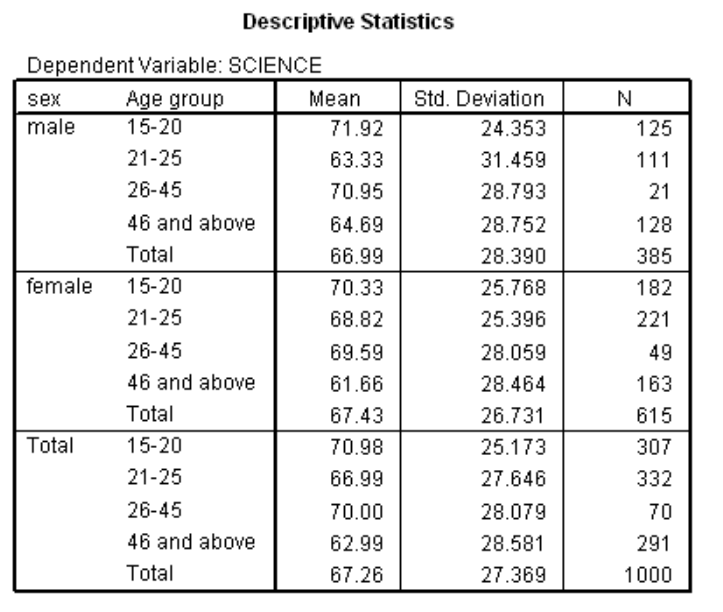
\includegraphics[width=0.65\linewidth]{images/SPSS-Week1}
%\end{figure}
\begin{enumerate}
\item What is the mean Science score for all Males?
\item What it the mean Science score for all Females?
\item What is the mean Science score for everybody in the study?
\item How many respondents are there altogether?
\item How many people are in the 15-20 age group altogether?
\item Which Age group has the highest Score?
%\item What is the smallest age group in the sample?
\end{enumerate}

\section*{Probability Distributions}


\begin{itemize}
\item The discrete uniform distribution
\item The continuous uniform distribution
\item The binomial disribution
\item The poisson distribution
\item The exponential distribution
\item the Normal distribution
\end{itemize}



%\begin{enumerate}
%%--Distributions
%
%
%
%
%\item uniform - The lower and upper bounds are 13cm and 21cm respectively.
%
%\item A computer server breaks down, on average, once every three months.
\begin{itemize}
\item What is the probability that the server breaks down three times in a quarter?
\item What is the probability that a server breaks down exactly five times in one year?
\end{itemize}

Assume that the number of weekly study hours for students at a certain university
is approximately normally distributed with a mean of 22 and a standard deviation
of 6.
\begin{itemize}
\item Find the probability that a randomly chosen student studies less than 12
hours.
\item Estimate the percentage of students that study more than 37 hours.
\end{itemize}


%A charity believes that when it puts out an appeal for charitable donations the donations it receives 
%will normally distributed with a mean 50 and 
%
%standard deviation €6, and
%
% it is assumed that donations will be independent of each other.
%
%\begin{itemize} 
%\item Find the probability that the first donation it receives will be less than€40.
%
%\item Compute the probability that it will be between €40and €45.
%\item Compute the value $x$ such that 5\% of donations are more than €$x$.
%\end{itemize}
%
In an examination the scores of students who attend schools of type A are
normally distributed about a mean of 55 with a standard deviation of 6. The
scores of students who attend type B schools are normally distributed about a
mean of 60 with a standard deviation of 5.
Which type of school would have a higher proportion of students with marks above 70?

The heights for a group of forty rowing club members are tabulated as follows;

\begin{table}[ht]
\begin{center}
\begin{tabular}{|rrrrrrrrrr|}

\hline
141 & 148 & 149 & 149 & 155 & 156 & 167 & 169 & 169 & 170 \\
171 & 173 & 175 & 176 & 177 & 179 & 182 & 182 & 183 & 183 \\
183 & 184 & 184 & 184 & 185 & 185 & 185 & 186 & 186 & 189 \\
191 & 191 & 191 & 191 & 192 & 192 & 192 & 193 & 194 & 199 \\
\hline
\end{tabular}
\end{center}
\end{table}

%%%%%%%%%%%%%%%%%%%%%%%%%%%%%%%%%%5555

\begin{enumerate}
\item Summarize the data in the above table using a frequency table. Use 6 class intervals, with 140 as the lower limit of the first interval.
\item Draw a histogram for the above data.
\item Comment on the shape of the histogram. Based on the shape of the histogram, what is the best measure of centrality and variability?
\item Construct a box plot for the above data. Clearly demonstrate how all of the necessary values were computed.
\end{enumerate}


